%!TEX root = ../../main.tex
I dette afsnit ses de forskellige Use cases. På figur~\ref{fig:fullydressedusecases} vises et use-case diagram over de fully-dressed use-cases, som viser de use-cases, som er i fokus. På figur~\ref{fig:ikkefullydressedusecases} vises et use-case diagram over de ikke fully-dressed use-cases, som ønskes implementeret på et senere tidspunkt. 
\begin{figure}
	\centering
	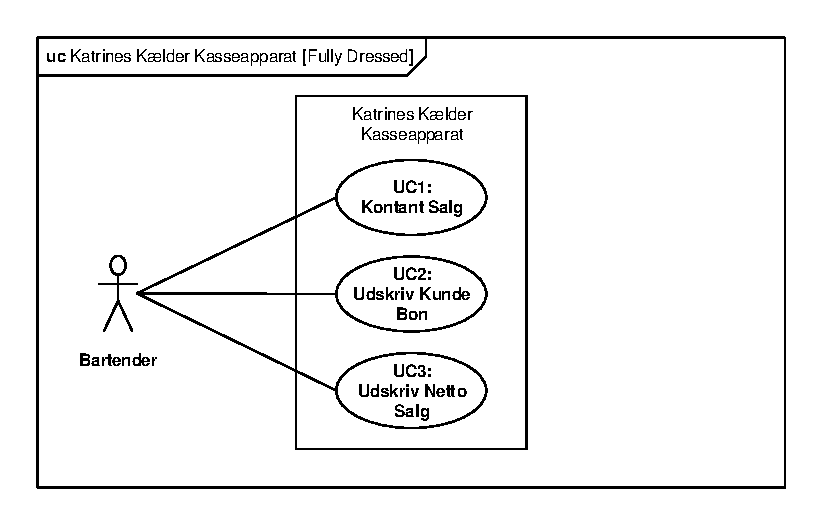
\includegraphics[width=0.8\textwidth, trim=5mm 5mm 5mm 5mm, clip, page=1]{Kravspecifikation/UseCases/Use-cases.pdf}
	\caption{Use-case diagram for de fully dressed use-cases.}
	\label{fig:fullydressedusecases}
\end{figure}

\begin{figure}
	\centering
	\includegraphics[width=0.8\textwidth, trim=5mm 5mm 5mm 5mm, clip, page=2]{Kravspecifikation/UseCases/Use-cases.pdf}
	\caption{Use-case diagram for de ikke fully dressed use-cases.}
	\label{fig:ikkefullydressedusecases}
\end{figure}
\newpage